\chapter{آزمایش‌ها}
برای بررسی عملکرد الگوریتم تی-اس-ای \LTRfootnote{t-SNE}  با دیگر الگوریتم‌های زیر مورد مقایسه قرار داده شده است.
\begin{itemize}
	\item $Sammon mapping$
	\item $Isomap$
	\item $LLE$
	\item $CCA$
	\item $SNE$
	\item $MVU$
	\item $ Laplacian Eigenmaps.$
\end{itemize}
این مقایسه برای پنج دیتاست انجام شده که در مقاله به سه مجموعه داده اشاره می‌شود که در زیر آورده شده است.
\section{دیتاست‌ها}
پنج دیتاستی که مقایسه روی آن‌ها انجام شده است عبارتند از :
\begin{itemize}
	\item دیتاست $MNIST$
	\item دیتاست $Olivetti faces$
	\item دیتاست $COIL\-20$
	\item دیتاست مربوط به کلمات.
	\item دیتاست نتفلیکس.
\end{itemize}.
\\
در این بخش سه دیتاست اول را مورد بررسی قرار میدهیم. 
\\
دیتاست اول دارای شصت‌هزار عکس از اعداد دست‌نوشته می‌باشد. برای این‌ آزمایش شش ‌هزار تصویر به صورت تصادفی برای بار محاسبتی کمتر انتخاب شده اند. هر تصویر شامل ۷۶۸ پیکسل می‌باشد.دیتاست دوم شامل ۴۰۰ تصویر از ۴۰ لیوان مختلف از هر لیوان ۱۰ تصویر و هر تصویر دارای ۱۰۳۰۴ پیکسل می‌باشد که هر تصویر با توجه به مشخصاتی که دارا بود برچسب خورده است. دیتاست سوم نیز شامل ۱۴۴۰ تصویر با ابعاد ۳۲ در ۳۲ می‌باشد که از ۲۰ شی مختلف تصویر برداری شده است.

\section{نحوه‌آزمایش}
در این آزمایش در ابتدا همه دیتاست‌ها با استفاده از $pca$ به ۳۰ بعد کاهش یافته اند. این کار به دلیل بار محساباتی کمتر صورت گرفته است. همچنین همه نقاط در سه دیتاست رنگ‌بندی شده اند. این رنگ بندی صرف فهمیدن بهتر نحوه عملکرد الگوریتم‌ها صورت گرفته است.
\\
پارامتر‌های تابع هزینه هر الگوریتم در زیر معرفی شده است.
\begin{itemize}
	\item الگوریتم $t\-SNE$: در این الگوریتم پارامتر سرگشتی توزیع شرطی احتمال که توسط کرنل گوسی استفاده شده برابر 40 قرار داده شده است.
	\item الگوریتم $sammon mapping$: در این الگوریتم متد نیوتون با ۵۰۰ بار تکرار انجام شده است..
	\item الگوریتم $Isomap$ و $LLE$ : در این دو الگوریتم عدد $k$  مربوط به تعداد همسایگان نزدیک در گراف همسایگی ۱۲ در نظر گرفته شده است.
\end{itemize}.
\\
\section*{نتایج}
در زیر تصاویر مربوط به نتایج آورده شده است .تصاویر به وضوح عملکرد مناسب$t\-SNE$ را نشان‌میدهد در به‌صورتی که تصویر مربوط به دیتاست اول دو الگوریتم $ISomap$ و $LLE$ باعث شده‌اند داده‌ها در بعد پایین هم‌پوشانی بالایی داشته‌باشند اما در الگوریتم $sammon mapping$ تنها سه کلاس از داده های کلاستر شده از‌هم جدا باشند و دیگر داده‌ها مشابه شوند ولی در مقابل الگوریتم معرفی شده توانسته است تا حد قابل قبولی داده‌های مشابه را نسب به دیگر داده‌ها نزدیک تر قرار دهد.

\begin{figure}
	\centering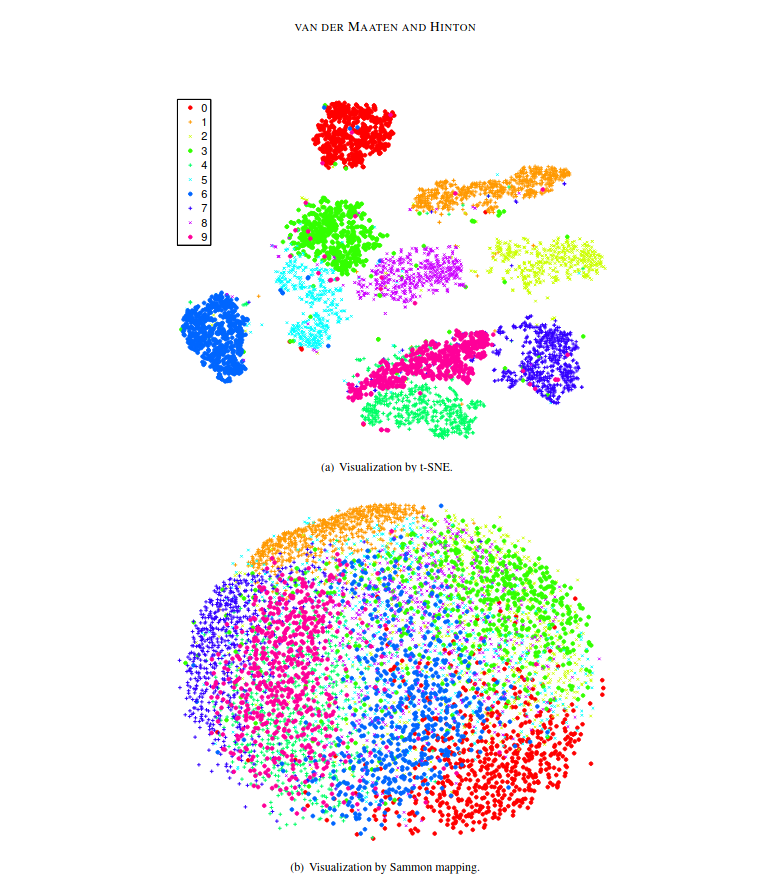
\includegraphics[scale=.6]{resfig1.png}
	\caption{نمایش ۶۰۰۰ هزار تصویر اعداد ۱ تا ۹ به صورت دست‌نویس از دیتاست اول}\label{resfig.1}
\end{figure}

\begin{figure}
	\centering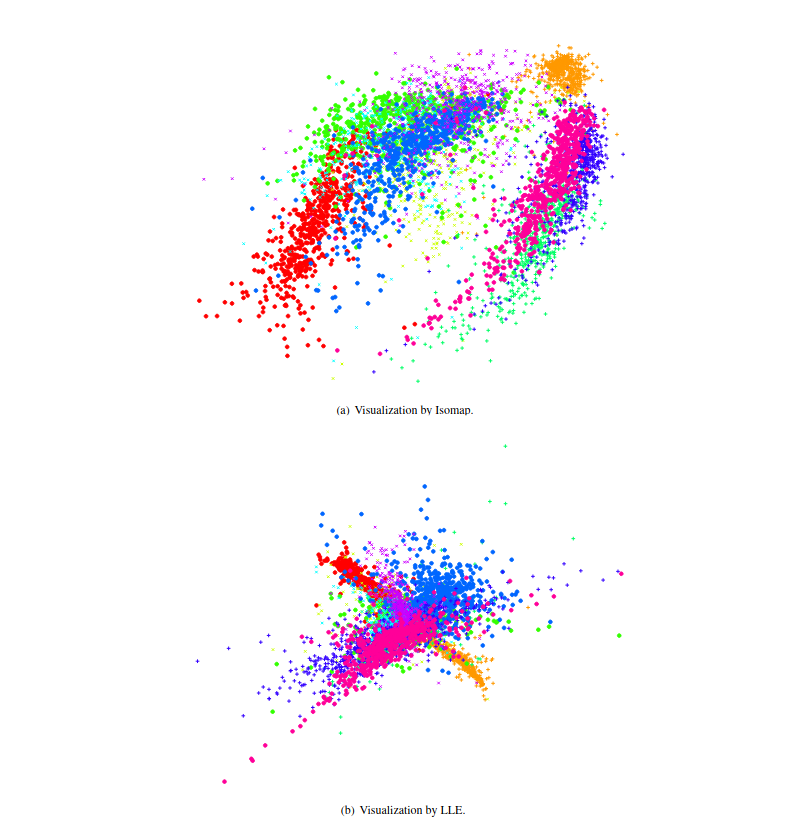
\includegraphics[scale=.6]{resfig2.png}
	\caption{نمایش ۶۰۰۰ هزار تصویر اعداد ۱ تا ۹ به صورت دست‌نویس از دیتاست اول}\label{resfig.2}
\end{figure}

\begin{figure}
	\centering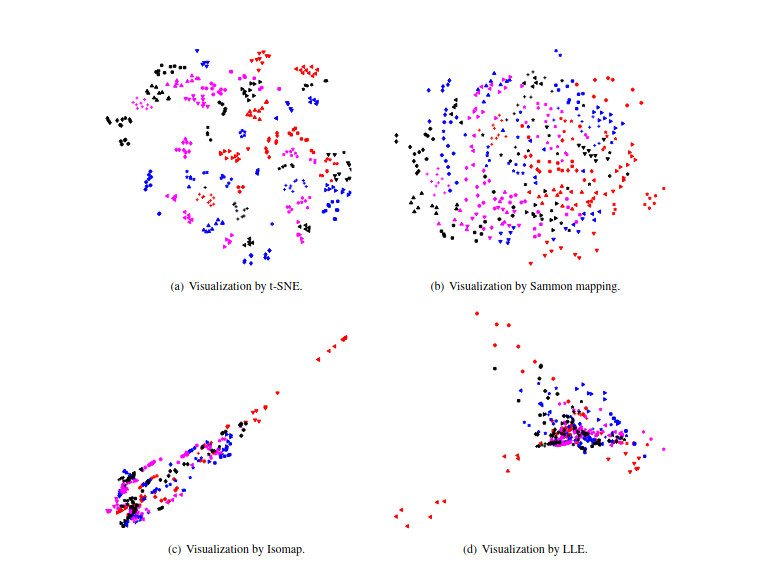
\includegraphics[scale=.6]{resfig3.png}
	\caption{مقایسه الگوریتم‌ها در دیتاست دوم}\label{resfig.3}
\end{figure}

\begin{figure}
	\centering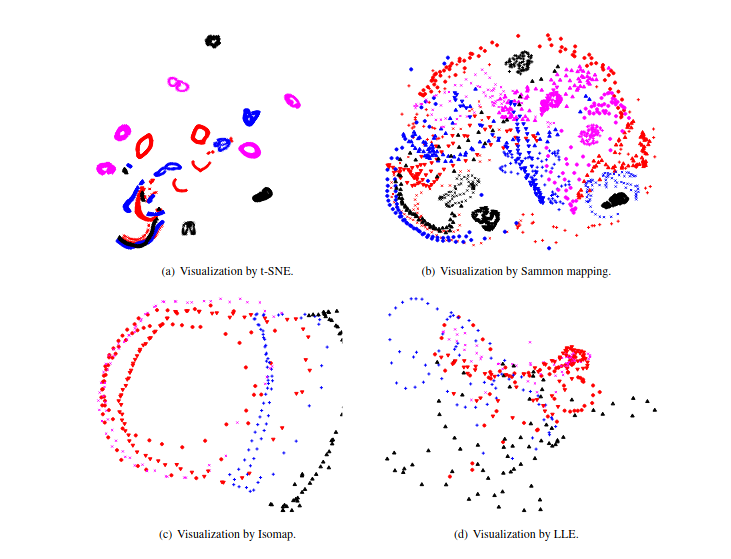
\includegraphics[scale=.6]{resfig4.png}
	\caption{مقایسه الگوریتم‌ها در دیتاست سوم}\label{resfig.4}
\end{figure}
سه مقایسه بالا نشان داد دیگر الگوریتم‌ها به خوبی $t\-SNE$ معرفی شده کار نمی‌کنند همچنین لازم به ذکر است که با توجه به محاسبات الگوریتم‌های $Isomap$ و  $LLE$  در دیتاست دوم ، اعداد حاصل در نزدیک بودن کلاس‌های معرفی شده بسیار بزرگ بوده و باعث شده‌است که حتی نتواند انها در  داخل یک دسته نگه دارد.

